\section{降维检验与环境敏感性}
\subsection{中截面、端部与整根积分}
中截面配对需要保持相同物性、环境与边界，才能识别额外轴向交换的影响。问题一80$\times$128二维对照在0--1800\unit{s}中截面采样的最大温度差约为$5.65\times10^{-8}\unit K$，含水率差约为$4.09\times10^{-9}\unit{kg/kg}$。问题二采用最终80$\times$256对照，在前10800\unit{s}的对应差为$1.69165\times10^{-3}\unit K$与$2.24706\times10^{-5}\unit{kg/kg}$，支持中截面工程近似，但不能宣称所有四位单元均一致。

另一方面，端面交换会改变整根失水。按二维控制体权重与一维圆环权重积分得到表\ref{tab:wholebody}。表中“失水增加”定义为$(C_0-\overline C_{2D})/(C_0-\overline C_{1D})-1$，不是平均含水率的相对误差。在空间均匀干密度的共同假设下，体积权重平均等于干质量权重平均。
\begin{table}[htbp]
\centering\small
\caption{同网格保存场的整根失水对照}\label{tab:wholebody}
\begin{tabular}{@{}lrrrr@{}}
\toprule 情形与时刻&二维网格&$\overline C_{2D}$&$\overline C_{1D}$&失水增加/\%\\\midrule
问题一，1800\unit{s}&80$\times$128&2.274929&2.293532&7.2533\\
问题二，3\unit{h}&80$\times$256&1.327482&1.382492&4.7118\\
问题四，6\unit{h}&80$\times$128&1.024545&1.065198&2.7379\\
\bottomrule
\end{tabular}
\end{table}
\FloatBarrier
中截面差小与整根总量差可见并不矛盾。若用于全长平均、总失水或端部状态，应采用二维积分或明确忽略端面的近似，不能把中截面表格的精度扩展到全部工程指标。

打开端面后，配对算例显示最湿点更早达到阈值，但这尚不是一般比较定理。温度场与含水率相互耦合；即使$D$随温度增加，两个解之间的变系数通量散度也未必具有统一符号。因此问题三、四的一维执行值、二维节点场、配对校正与连续严格界分别报告。

\subsection{后段环境的受控情景}
由于式\eqref{eq:future}仅为4\unit{h}后的延拓，保持短时实测过程不变，从保存的4\unit{h}内部温湿场开展后段联立续算。每问设置原平台、温度$\pm1\unit K$和有效边界$b\pm0.005$五种情景；第四问始终使用同一观测$R(t)$。扰动幅度为人为选择的压力测试，没有作为测量不确定度或置信区间。表\ref{tab:environment}给出40阶配点的等号事件根，差值相对于同阶基线。
\begin{table}[htbp]
\centering\small
\caption{4\unit{h}后环境改变的条件根与时长差}\label{tab:environment}
\begin{tabular}{@{}lrrrr@{}}
\toprule 情景&问题三根/h&变化/h&问题四根/h&变化/h\\\midrule
原均值平台&57.473996&0&51.092003&0\\
$T_a-1\unit K$&59.341275&$+1.867279$&52.729346&$+1.637343$\\
$T_a+1\unit K$&55.688357&$-1.785639$&49.525343&$-1.566660$\\
$b-0.005$&57.382748&$-0.091249$&50.993818&$-0.098185$\\
$b+0.005$&57.584113&$+0.110117$&51.218753&$+0.126750$\\
\bottomrule
\end{tabular}
\end{table}
\begin{figure}[htbp]
\centering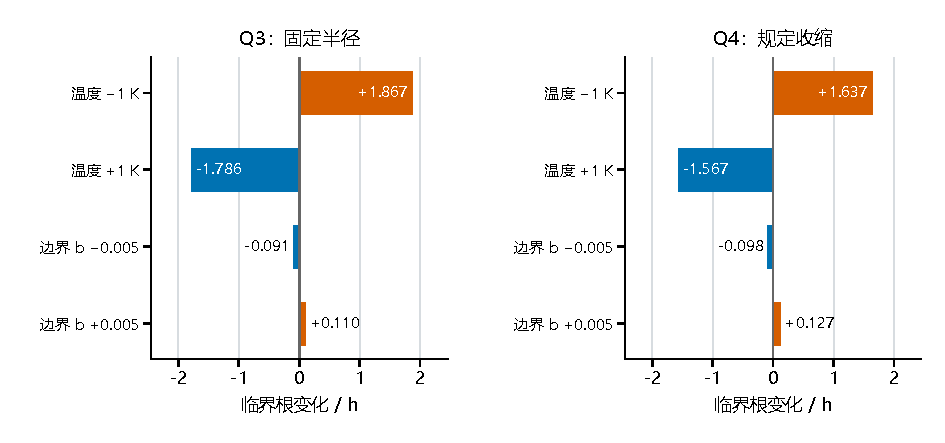
\includegraphics[width=.93\linewidth]{figures/environment_sensitivity.pdf}
\caption{后段环境情景相对同阶基线的根变化；幅度为人工设定，第四问规定半径保持不变。}\label{fig:environment}
\end{figure}
\FloatBarrier

对基线和降1\unit K情景进一步加密：问题三40阶到80阶、问题四40阶到60阶，单个根的最大变化分别约0.002951\unit{s}与0.000174\unit{s}，降温净效应的变化更小。因此小时级差不是此次降阶造成的；其他扰动没有逐一加密，表中六位小数仅便于追踪数值，不代表真实预测精度。

长期降温在既定模型内减小扩散温度因子，推迟阈值；提高$b$减小失水驱动力，也使根后移。由于两类扰动尺度不同，不能据图\ref{fig:environment}断定温度比所有湿度误差都重要。已有时间加权均值对照使问题三根变化约20.04\unit{s}，问题四改用PCHIP半径插值使根提前约12.61\unit{s}，二者也超过亚秒级一维经验数值预算。工程执行余量应建立在可用工况范围上，不能只依据四位小时的取整步长。

\section{模型适用范围与改进方向}
\subsection{气固边界与目标可达性}
材料$C$和空气$y_a$虽然都可写作\unit{kg/kg}，分母却未必相同。湿空气湿度比、相对湿度和体积蒸气浓度需分别定义\cite{ashrae}。真实气膜候选边界可写为
\begin{equation}
j_s=k_g\{c_{v,s}(C_s,T_s)-c_{v,a}\},
\label{eq:physical-interface}
\end{equation}
其中$c_{v,s}$需材料水活度或解吸关系。若将浓度差局部线性化为$c_{v,s}-c_{v,a}\approx K(C_s-b)$，才能建立$\rhod h_m=k_gK$的对应，而非直接交换系数数值。圆柱有效干燥模型与移动边界模型分别使用平衡干基含水率或气相/解吸关系\cite{dasilva2014,adrover2020}，它们没有提供本药材的标定值。

首先需要核实目标环境下的材料平衡含水率$C_{\mathrm{eq}}$是否低于0.15。若恒定环境对应$C_{\mathrm{eq}}\ge0.15$，从较高含水率开始的扩散干燥可能无法实现全域严格阈值；提高网格精度不能消除这一不可达性。缺少数据时可报告边界情景，但不能给未经标定的$C_{\mathrm{eq}}$冠以实测含义。

\subsection{经验密度与材料质量的相容性}
若同时把题给$\rho=a+b_\rho C$解释为真实当前湿体密度，则干基定义要求
\begin{equation}
\rhod(C)=\frac{a+b_\rho C}{1+C},\qquad
\frac{\dd\rhod}{\dd C}=\frac{b_\rho-a}{(1+C)^2}.
\end{equation}
前三问固定骨架的干密度应保持不变，而该经验关系随失水改变；第四问仿射材料收缩要求$\rhod$空间均匀，但非均匀$C$会给出非均匀经验干密度。本文将题给$\rho$仅用于有效容量，是对上述不相容关系的建模处置，不能说题面已经规定了这一有效化解释。

以第四问保存场作反证性积分，若强制采用真实湿密度解释，则7\unit{h}和末态的隐含干质量相对初值分别为0.71952、0.89029。保持现有$C,R$场不变，只靠改变长度凑足总干质量，需由25\unit{cm}增至34.7454\unit{cm}与28.0807\unit{cm}。这说明增加轴向收缩不能修复当前缺口；即使伸长凑平总量，局部相容性仍待解决。该诊断不等于本文独立干质量账本发生了数值泄漏，也不是新的可行伸长模型。

\subsection{相变能量与可报告的指标}
式\eqref{eq:heat}只描述有效温升，不含显式潜热。有限的$\rhoe c_p$不能在近等温而持续失水时自动补充汽化功率。为考察量级，在“初始湿密度确定干质量、全部等效失水均蒸发”的附加条件下，取诊断常数$\lambda=2.45\unit{MJ/kg}$\cite{fao}，问题一1800\unit{s}的潜热需求约45.59\unit{kJ}，原温度轨迹对流输入约4.801\unit{kJ}，比例约9.50。

问题四12\unit{h}表面温度几乎等于环境，原轨迹净对流输入接近零，而条件潜热通量$\lambda\rhod h_m(C_s-b)$约164.10\unit{W/m^2}。这一反例足以排除“题给有限$c_p$已自动包含潜热”的解释，但不是实际耗能测量。若重新联立相变，表面降温会增加热输入并改变扩散，不能拿原热输入固定不变直接倍乘干燥时间。

因此本文可报告题给有效模型的温湿分布、阈值事件和条件时长差，不能从中推出实际节能率或真实执行保证。进一步闭合应让同一真实$j_s$进入质量与能量边界，并采用一致焓基准；域内含水率下降包含水分扩散，不能全部视为局部蒸发，再重复加入体积潜热项。

\subsection{优先补强的计算与数据}
数值层面，最直接的补强是第四问正式时刻的精细二维场，配合径向加密、时间紧化及起点前史误差检查，使正阈值裕量覆盖相称误差。仅把粗网格晚期场插值到细网格，不能消除共同继承偏差；普通收敛检验也不同于连续数学误差界。

模型层面，优先比较“固定干基$h_m$”与“固定$\rhod h_m$”的条件响应，再用实测后段环境建立适用工况。若有独立失重和表面温度数据，先在短时窗核查气固关系、干质量与相变能量，验证后再延长全过程。仅有$R(t)$是边界输入，不能据其吻合宣称温湿预测或其他工况的收缩反馈已获实验验证。附录3/4与固定/收缩几何的第四格对照、非均匀材料运动可作为进一步研究，不应抢先于这些关键接口。
